\scanpage{101}
9/ \uline{Retour sur le cas} $\alpha=2$, $\alpha\ne-2$ (i.e. $\alpha=2$ en car. $\ne2$).

On a
\[
f(x,y)=(\deleted{\unsure{x^2}}x-y)^2-(x+y)=v^2-w
\]
\[
\text{où}\qquad
\left\{\begin{aligned}v&=x-y\\w&=x+y\end{aligned}\right.
\quad\text{i.e.}\quad
\begin{aligned}x&=\tfrac12(\unsure{v|w}+w)\\y&=\tfrac12(-v+w)\end{aligned}
\]
Le calcul donne pour $u$, défini en coordonnées \unsure{universelles|anciennes} par
\figure{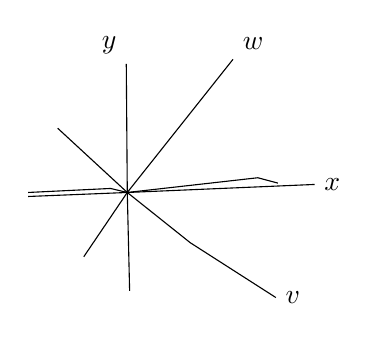
\begin{tikzpicture}[x=.85cm,y=.85cm]
\draw (-1.48,-.06) -- (0,0) -- (2.80,.12) node[right] {$x$};
\draw (-1.48,0) -- (-.25,.06) -- (0,0) -- (1.95,.22) -- (2.25,.14);
\draw (.035,-1.47) -- (0,0) -- (-.015,1.92) node[above left] {$y$};
\draw (-.65,-.96) -- (0,0) -- (1.58,1.99) node[above right] {$w$};
\draw (-1.04,.96) -- (0,0) -- (.94,-.75) -- (2.22,-1.57) node[right] {$v$};
\end{tikzpicture}}
\[
u(x,y)=(1-y+2x,x)
\]
en coordonnées $(v,w)$
\[
U(v,w)=(v+1,1+2v+w)
\]
en particulier, pour des points sur la parabole $C(f)$ d'équation ${\unsure{w|v}}^2-\unsure{v|w}=0$ i.e. $w=v^2$
\[
U(v,v^2)=\deleted{(\unsure{v+1,1+}}\,(v+1,(v+1)^2).
\]
Donc si on paramètre $C(f)$ par la coordonnée $v$, alors $u\mid C(f)$ est décrit par la translation $v\mathrel{\unsure{\mapstochar\relbar\mapstochar|\mapsto}}v+1$ !
% archive sheet number: 100
